\chapter{Conclusions and Future Work}
\label{ch:concl}

This chapter focuses on concluding remarks and future work.  First in Section
\ref{sec:concl}, the main experimental results from each section are brought
together to discuss the bigger picture of this work.  Additionally, there are
areas of the methodology that are simplified and several avenues this work
could pursue, so this is discussed in Section \ref{sec:future}.

\section{Conclusions}
\label{sec:concl}

The main research question that this work addresses is as follows: \textit{How
does the ability to determine forensic-relevant spent nuclear fuel attributes
using machine-learning techniques degrade as less information is available?}. 
The workflow to examine this question takes place in four steps.  

First, the training data is simulated, which provides an array of nuclide
measurements as the features. The prediction parameters are the simulation
inputs: reactor type, burnup, \gls{U235} enrichment, and time since
irradiation.  The reactor types are one of three common commercial reactors:
\gls{PWR}, \gls{BWR}, or \gls{PHWR}.  The burnup is measured in $MWd/MTU$ , the
enrichment is measured in $\%{}^{235}\text{U}$, and the time since irradiation
is measured in $days$. The size of the training set is $4.5 \times 10^5$
\gls{SNF} entries, which were simulated using \gls{ORIGEN} \cite{scale, origen,
origenarp}.  These steps are covered in Sections \ref{sec:training1} and
\ref{sec:training2}.

Second, information reduction on the training set is carried out using randomly
injected uniform error or computationally generated gamma spectra. For the
former, the training set is comprised of nuclide masses and the random error is
used to study the robustness of the methodology to artificial noise in the
feature set.  For the latter, the training set becomes lists of summed energy
windows of the gamma spectra, which were computed from nuclide activity
measurements using \gls{GADRAS} \gls{DRF}s for six detectors \cite{gadras}.
Each detector-based training set undergoes three different methods of
processing the gamma spectra, denoted as auto, short, and long energy windows
lists.  These steps are covered in Sections \ref{sec:inforeduc1} and
\ref{sec:inforeduc2}.

Third, three algorithms are used to predict the four reactor operation
parameters in this work: \textit{k}-nearest neighbors, decision trees, from the
scikit-learn python \gls{ML} toolkit, and \gls{MLL} calculations, implemented
in python using SciPy and NumPy \cite{scikit, scipy, numpy}.  For the scikit
algorithms, the hyperparameters governing model complexity were optimized to
minimize the prediction errors.  All of the code was run using
\gls{UW}--Madison's \gls{CHTC} resources, the \gls{UW} campus grid, and the
\gls{OSG} \cite{osg07, osg09}.  These steps are covered in Sections
\ref{sec:statmodel1} and \ref{sec:statmodel2}.

Fourth, the prediction errors are evaluated to understand the increase in error
as the information supplied is less precise. This impacts the conclusions that
can be formed about the capability of simple statistical methods to inform
nuclear material attribution.  The testing samples come directly from the
training set, and the prediction errors from  these testing sample are what is
studied for the performance.  When a test sample is used, it is first removed
from the training set so that there is no exact replica of it in the training
stage.  This testing scheme allows the entire training set to be tested
eventually.  It is accomplished via 5-fold \gls{CV} for the scikit-learn
algorithms and by testing one training set entry at a time for the \gls{MLL}
calculations.  These results are presented in Sections \ref{sec:eval1} and
\ref{sec:eval2}, and are summarized as follows.

\noindent \textbf{Reactor Parameter Prediction Using Nuclide Masses}

Here, the results from the experimental procedure in Chapter \ref{ch:exp1} are
discussed.  This experiment is a demonstration of the methodology with the
"perfect knowledge" of nuclide masses. Information reduction is accomplished by
adding noise to the training set in the form of randomly applied uniform error.
The results are in Sections \ref{sec:randerrA} and \ref{sec:randerrB}.  In
order to understand the ability of the models to generalize, the performance
with respect to training set size is studied in Section \ref{sec:randerrC}.
Section \ref{sec:randerrD} introduces the impacts of having prior knowledge of
the reactor type on the quality of prediction of the regression cases.  Last,
the external testing set, the \gls{SFCOMPO} database, is used to test this
methodology against sometimes complicated real world data sets in Section
\ref{sec:sfcompo}. 

Sections \ref{sec:randerrA} and \ref{sec:randerrB} demonstrate the impacts of
injected training set noise on the prediction parameters. Aside from the
\textit{k}-nearest neighbors prediction of time since irradiation, all of the
algorithms follow a similar pattern for each prediction scenario.  The
\gls{MLL} calculations are the most resilient to introduced error, followed by
decision trees then \textit{k}-nearest neighbors.  It is difficult to state
whether or not these results are "good enough" on their own, but they do serve
as a useful baseline for the results in Chapter \ref{ch:exp2}. 

Next, the model generalization is studied in Section \ref{sec:randerrC} by
creating learning curves using $20-100\%$ of the training set.  It shows that
the training set is large enough for the \gls{MLL} calculations to remain the
best performing until the 20\% level, when those data points dip below one or
both of the scikit-learn algorithms depending on the prediction parameter. It
should be noted that this performance is highly dependent on the training set
design because these are qualitatively high variance methods (compared to
common algorithms not shown in this work) that do not generalize well. 

Section \ref{sec:randerrD} investigates the effect of having reactor type prior
knowledge on burnup, enrichment, and time since irradiation prediction.  There
is modest and significant improvement for \gls{PWR} and \gls{PHWR} cases,
respectively, since they are both the minority classes in the training set.
These improvements only exist for the scikit-learn algorithms, since the
\gls{MLL} calculations are not affected by reactor type knowledge.

The last study in this chapter is in Section \ref{sec:sfcompo}, where an
external test set is used that is comprised of measurements from real
commercial power \gls{SNF} from around the world: the \gls{SFCOMPO} database.
The main challenge with this database are that many entries only contain
measurements for uranium and plutonium isotopes, and the missing measurements
are inconsistent. Two methods were implemented: imputing the null values and
replacing the null values with zero.  The reactor type classification results
are very poor except for the \gls{MLL} predictions using zero-valued nulls.
This combination also best predicts the burnup, but oddly, the decision trees
for both methods of null handling best predicts the enrichment.  The
techniques for improving the performance are discussed next in the future work
suggestions, Section \ref{sec:future}.

\noindent \textbf{Reactor Parameter Prediction Using Processed Gamma Spectra}

Next the results of the second experimental procedure from Chapter
\ref{ch:exp2} are discussed.  This experiment's purpose is to probe the
usefulness of field-deployable detectors for giving rapid information about
presumed \gls{SNF}. The information reduction is achieved by using
computational gamma spectra of various detectors with decreasing detector
energy resolution.  The gamma spectra of each \gls{SNF} entry are
processed in three different manners, resulting in three energy windows lists,
denoted by auto, short, and long.  

The reactor type classification results are first covered in Section
\ref{sec:exp2_rxtr}.  Unsurprisingly, the \gls{MLL} calculations consistently
perform the best across the algorithms. There is a slightly better overall
performance by the short energy windows list as compared to the others,
although the large variation by the auto energy windows lists has some data
points performing better.  The confusion matrices show the details of every
data point, but most of the misclassifications are \gls{PWR} and \gls{PHWR} being
labeled as \gls{BWR}.  The automatic peak searching results in erratic behavior
for the scikit-learn algorithms, noting the poor performance of the high energy
resolution detectors, presumably from the added noise of including all peaks
instead of just targeted peaks like the other two lists.  It is still a
promising approach for the lower energy resolution detectors, and possibly even
the high energy resolution detectors since in theory one could filter the noise
from the detector peak searches. 

Next, the regression cases are shown in Section \ref{sec:exp2_reg}.  Regardless
of the energy windows list, the detector-based training sets all do the
following for the \gls{MAPE} and \gls{MAE}: the burnup tends to far outperform
the baseline, the enrichment consistently underperforms with respect to the
baseline, and the time since irradiation has values along the baseline, where
many are below line but close to it.  The spread of absolute errors including
the outliers shows that there is a significant portion of the training set that
is being predicted with very large errors; the spread of outliers encompassed
$3-17\%$ of the training set depending on the case.  Studying these results
with respect to the \gls{MedAE}, the burnup and time since irradiation
predictions do well with respect to their baselines. 

\noindent \textbf{Post-Summary Statements}

There is a clear leader throughout all of the results in terms of being a
consistent best performer: the \gls{MLL} calculations. The reason it can
perform well, though, is because of the large number of simulations.  The time
steps in the training set being about $100\:days$ was a limiting factor in its
quality of prediction; many of the \gls{MAE} values were around this level in
the second experiment. The poor enrichment prediction is likely because the
detected radionuclides are not enrichment indicators \todo{check}, and despite
many of the nuclides that are included in the short and long energy windows
lists having known poor simulation quality, the burnup prediction clearly had
enough information to do well.  If there were to be a training set of much
higher fidelity but larger steps between the training set labels, it is
possible \gls{MLL} would not be a top performer. 

The two scikit-learn algorithms still had some interesting variation in their
prediction capabilities despite usually under-performing. Decision trees best
predicted the enrichment for the external testing set scenario with
\gls{SFCOMPO}. For all of the 0\% training set error cases in the first
experiment, the scikit-learn algorithms performed better.  The \gls{MLL}
robustness to error is likely from the different manners in which the error was
applied.  The scikit-learn approach was to change the training set feature
itself to a new value within some range based on the error, but the \gls{MLL}
approach was to include this error instead as uncertainty. In this way, it is
not affecting the features directly, just the resulting uncertainty of the
log-likelihood calculation. If the same approach was used, or some error
existed in the measurements, \gls{MLL} again might not be the best choice. 

Another way in which the implementation differed was the 5-fold \gls{CV} being
used as the testing protocol for the scikit-learn algorithms. For 5 rounds,
20\% of the training set is removed as a testing set, where eventually all 5
folds are tested.  By contrast, the \gls{MLL} test samples get removed a single
entry at a time.  If the training set were to be more sparsely populated with
the same range of each label, this would be of larger concern.  From the
learning curves in Figure \ref{fig:learns}, it appears that reducing the
training set by 20\% would in theory not impact the \gls{MLL} performance, but
it is still a major difference in implementation. 

Note for nuclides: feature importance work gave different lists for each label,
but since each training set is designed to be able to predict all four
different labels, not all features are relevant to a given label. This adds a
lot of noise for a given label prediction. 

With respect to the number of features affecting the prediction performance,
the overall similarity of performance among the three energy windows lists
might mean that the feature numbers are not impacting the algorithms much.
Another explanation is that they all include too many features (outside of the
scintillator detectors with the auto energy windows list).  It is possible that
even the short list with 42 features has too high of a dimension for these
methods to perform well. \todo{unfinished}

Reminder than equal error in training and testing is not realistic. Training
data should be as perfect as possible bc its stagnant

\section{Future Work}
\label{sec:future}

When designing any study, simplifications and assumptions must be made to take
a first-order look at the problem. Additionally, any good exploration is likely
to generate more questions than answers. This final section covers a list of
future work based on the the simplifications made and questions created.

\subsection{Training Set Features}

\noindent \textbf{Simulation Fidelity}

\gls{ORIGEN-ARP} not only offers computational expediency, but the training set
creation was able to be fully scripted and automatically carried out. The $4.5
\times 10^5$ entries in the training set were simulated in a matter of hours on
a personal computer.  

Section \ref{sec:fidelity} discusses the fidelity of the simulations used to
create the training database, and how the ground truth in this work is
therefore not perfect truth.  The first improvement to be made with the
training set is filtering out problematic-to-simulate nuclides, such as
${}{125}\text{Sb}$. An exercise was carried out to compare \gls{ORIGEN-ARP}
simulations to an entry in \gls{SFCOMPO}, and there were some nuclide
discrepancies that reached 40\%. It would be better to remove these from
consideration if they are systematically poorly simulated.

One level beyond this would be to forego the convenience that \gls{ORIGEN-ARP}
provides and use higher fidelity simulations in \gls{SCALE}. 

\noindent \textbf{Feature Set Study}

The lists of training set features in this work were not chosen based on
knowledge of nuclear reactor operation and the best signatures for the various
labels being predicted (reactor type, burnup, ${}^{235}\text{U}$ enrichment,
time since irradiation).  Instead, they were chosen based on the nuclide
availability in the \gls{SFCOMPO} database and the computational gamma spectra
tool, \gls{GADRAS}, which gave 29 and 32 nuclides, respectively. 

For the 29 nuclide mass training set, a small feature importance exercise was
carried out to determine if these lists could be reduced further. This was
carried out by using \texttt{SelectKBest(score\_func=f\_regression,
k=29).fit(X,y)} (or \texttt{f\_classif} for reactor type classification),
sorting the scores of the features, choosing the top $N$ features for each
label, and taking the set of features together for all labels.  The resulting
set of best-scoring features for all the labels included most or all of the
original list depending on the arbitrary decision of $N$.  This could be
further refined by combining domain knowledge of reactor physics and a more
structured statistical feature importance approach. Furthermore, because mass
spectrometry provides ratios of nuclides, studying how various ratios perform
versus nuclide masses or nuclide concentrations with respect to initial uranium
mass would be prudent. 

\noindent \textbf{Gamma Spectra Processing}

For the 32 nuclide activity training set, the most detectable gamma energies
emerged from the short and long energy windows lists to include from 7 and 12
nuclides, respectively, shown in Table \ref{tbl:enlistnucs}. So in this way,
nuclear physics performed the feature selection.  It is clear from the results
that the 7- and 12-nuclide lists performed quite well, and exceeded the
baseline for all four prediction scenarios.  However, there were many high
energy photopeaks excluded from these lists that might provide more
information. These were captured via the auto peak search method, but the
resulting energy windows list did not provide better results (and in some cases
with \textit{k}-nearest neighbors, provided worse performance).  This simple
approach should be refined with a study on the latest gamma spectra
processing tools. 

There are also more advanced detection techniques being studied, some which
could be simulated with \gls{GADRAS}.  This would provide easier peak
processing for nuclides of interest, e.g., with peaks at the high energy end of
the spectrum. \todo{finish}

Citations:

targeted or advanced measurement techniques \cite{snf_gamma, compton_supp,
bwr_high-res_gamma, pwr_bwr_gamma}

innovative spectra evaluation and radioisotope identification methods
\cite{riid_09, rapid_riid_18, sull_gen_07, sull_valid_15, sull_auto_17,
sull_unc_17}.

\subsection{Statistical Method Optimization}

The methods in this work all have high variance, and so it would have seemed
prudent to apply regularization. However, hyperparameter optimization did not
shift the high variance defaults much towards more bias.  The resulting
inability to generalize likely was a contributing factor to the large errors in
the results when using the \gls{SFCOMPO} database as a testing set. A closer
look at optimization is warranted in tandem with the above work on the feature
sets for each label.

Since the \gls{MLL} approach is essentially \textit{k}-nearest neighbors with
$k=1$ and a different loss metric, the \gls{MLL} calculations could be expanded
to include the option to have \textit{k} samples averaged for a response, which
would increase the bias.  Another option would be to use the likelihood
calculations as custom sample weights within the \textit{k}-nearest neighbors
algorithm. The implementation of \textit{k}-nearest neighbors in this work used
Manhattan distance $d_i$ with samples weighted by $1/d_i$. This would change
the sample weights to $L(M|x_{test})$, the likelihood as calculated in Equation
\ref{eq:like}.

It is entirely possible that optimizing the methods in this work can only
improve the prediction performance by a minimal amount, and that more complex
methods could be beneficial. \todo{finish}

\subsection{Serial Prediction}

Figure \ref{fig:knownrxtr} shows that for some combinations of prediction label
and algorithm, there is an improvement in the regression performance for the
\gls{PHWR} class, and less so for some \gls{PWR} cases.  (There was no
significant improvement seen for any reactor type/regression case combination
for the \gls{MLL} calculations.) Given the majority of the database is
comprised of \gls{BWR} entries, the improvement is not surprising; it is the
lack of improvement in the other cases that is unexpected. Either way, it makes
sense to first determine the reactor type before performing the other
predictions if not using the \gls{MLL} approach. One example of this being
done is in Reference \cite{serial_ml}.

Performing regression after first classifying the reactor type means much care
should be taken to have a robust reactor type classification algorithm. One way
to ensure better classification is by implementing a study that leverages
\gls{ROC} curves. \Gls{ROC} curves plot the true positive rate (vertical axis,
$\frac{\text{True Positives}}{\text{True Positives + False Negatives}}$) with
respect to the false positive rate (horizontal axis, $\frac{\text{False
Positives}}{\text{False Positives + True Negatives}}$) for various
\textit{decision thresholds}, as shown in Figure \ref{fig:roc} \cite{roc}.

\begin{figure}[!htb]
  \centering
  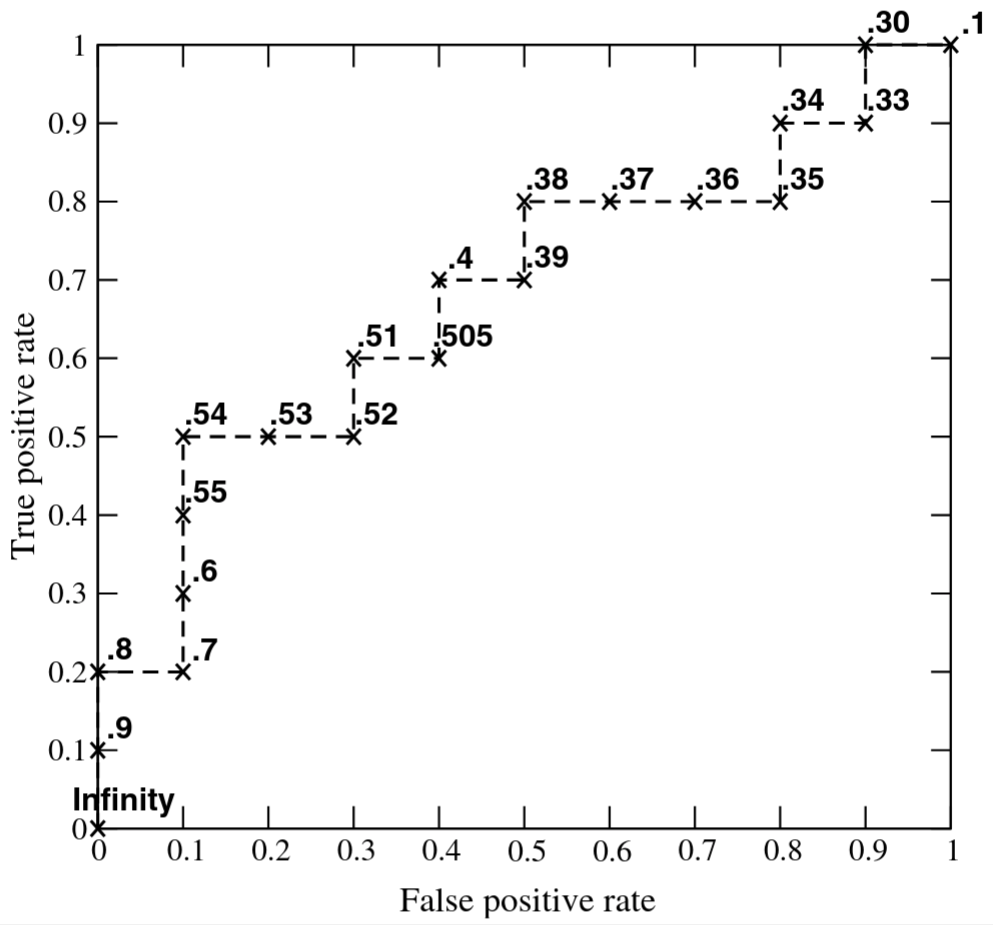
\includegraphics[width=0.8\linewidth]{./chapters/concl/roc.png}
  \caption[Example of an \acrshort{ROC} curve]
          {Example of an \acrshort{ROC} curve showing the decision threshold 
           (probability of class belonging) changing from $\infty$ to 0.1; this 
           is borrowed from Reference \cite{roc}.}
  \label{fig:roc}
\end{figure}

During prediction of a test sample, the scikit-learn classifiers calculate a
probability that the sample belongs to a given class. In binary prediction, the
default threshold is 0.5. A probability above this threshold means the sample
will be predicted to belong to the positive class, and below that the sample
will belong to the negative class.  In multi-class prediction, the highest
probability is chosen as the predicted class.

An ideal classifier would have values along the vertical axis and then straight
across the top, meaning beyond some threshold value there are zero false
positives. On the other end of the spectrum, if the classifier being used in
Figure \ref{fig:roc} were only choosing classes randomly, it would follow an
$x=y$ diagonal line. The one shown here performs somewhere in between these two
extremes. 

If the algorithm returns the probabilities of class belonging instead of the
predicted class, the threshold can be tuned after the fact to complete
predictions.  With this work, e.g., the decision threshold  could be manually
tuned to require a higher threshold for \gls{BWR} classification. If that were
the case, there could be fewer misclassifications of \glspl{PHWR}s and
\glspl{PWR}s as \glspl{BWR}s. The issues with regression of \glspl{PHWR}s could
then be resolved if they were accurately classified as such beforehand. T

\subsection{SFCOMPO}

The \gls{SFCOMPO} database being used as an external test set within the
framework of this methodology performed poorly in the sense that some relative
errors were extremely large. \todo{is this OK to say?} Section
\ref{sec:sfcompo} shows the results using two different methods for handling
the missing measurement values: imputation with the mean value of a given
nuclide, and replacing the null values with zero. 

One way to improve the results is using the previously discussed serial
prediction approach, where the reactor type is first determined before the
regression cases are predicted using training sets that only include entries
from the predicted reactor type.  This was partially touched on in Section
\ref{sec:sfcompo} by discussing the largest relative errors disappearing when
\glspl{PHWR}s were removed from consideration.  Another way that might improve
the results is with better simulation fidelity, also previously discussed. 

A third approach is revisiting the method by which the missing measurements are
handled.  One option is to side-step the missing nuclide measurements all
together.  Reducing the training set to only consider uranium and plutonium
isotopes accomplishes this; the majority of measurements in the training set
would exist and there would be very few missing measurements.  This is
essentially what the zero-valued nulls with \gls{MLL} calculations does, and
likely why it performed the best for the reactor type and burnup predictions
(and a close second for the ${}^{235}\text{U}$ enrichment prediction). 

Although the zero-null values approach is likely to always perform the best
with \gls{MLL} calculations, there are better approaches than mean (or median)
null value imputation. For example, one could take a \textit{k}-nearest
neighbors approach to imputation where the mean, median, or mode of the
\textit{k}-closest samples are used for imputation (rather than the mean,
median, or mode of the entire column in that testing set). Another approach for
handling missing values is outlined in Reference \cite{nf_missingdata}, where a
novel imputation approach for the \gls{SFCOMPO} database, called Monte Carlo
Bayesian Database Generation, is discussed.

